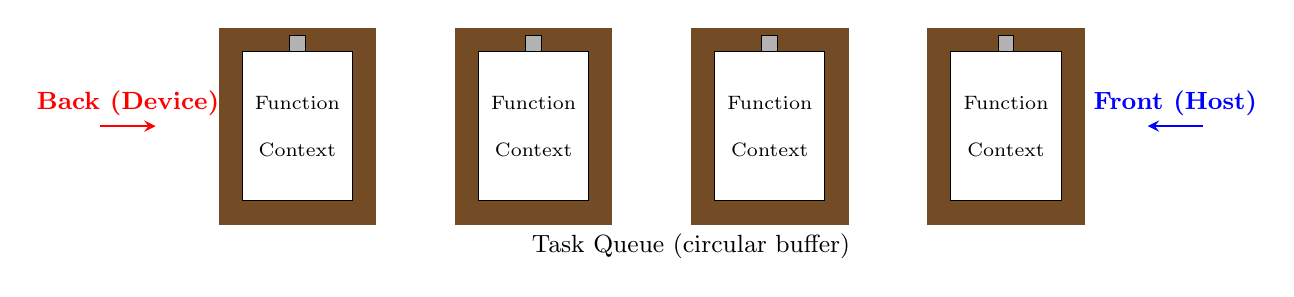
\begin{tikzpicture}[font=\small,>=stealth]

% Number of slots (more spacing)
\foreach \i in {0,1,2,3} {
    \pgfmathsetmacro{\x}{\i * 3} % spacing
    % Clipboard outer
    \fill[brown!60!black] (\x,0) rectangle (\x+2,2.5);
    % Inner white area
    \fill[white] (\x+0.3,0.3) rectangle (\x+1.7,2.2);
    \draw[black] (\x+0.3,0.3) rectangle (\x+1.7,2.2);
    % Gray clip area
    \fill[gray!60] (\x+0.9,2.4) rectangle (\x+1.1,2.2);
    \draw[black] (\x+0.9,2.4) rectangle (\x+1.1,2.2);
    
    % Labels inside
    \node[font=\scriptsize] at (\x+1,1.55) {Function};
    \node at (\x+1,0.95) {\scriptsize Context};
}

% Back pointer (Device) pointing to left side
\draw[thick,->,red] (-1.5,1.25) -- (-0.8,1.25) node[midway,above]{\textbf{Back (Device)}};

% Front pointer (Host) pointing to right side
\draw[thick,->,blue] (12.5,1.25) -- (11.8,1.25) node[midway,above]{\textbf{Front (Host)}};

% Label for queue
\node[below] at (6,0) {Task Queue (circular buffer)};

\end{tikzpicture}
